% \subsection{Synthetic Data}
% \subsubsection{Matrix Completion}
In this section, we evaluate \textsc{Hyper-SET} against vanilla Transformer and other baselines on discriminative and generative tasks. For fairness, we remove biases and dropout, use the Pre-Norm style with $\operatorname{RMSNorm}$, and set the MLP ratio to 4 in Transformer. We use one-layer trainable parameters but vary the forward iterations for all models, including Transformers, unless otherwise specified.\footnote{For instance, 12 iterations mean applying the layer repeatedly 12 times.}
% As one iteration of energy minimization corresponds to a single-layer update of tokens in \textsc{Hyper-SET}, we use one-layer trainable parameters but vary the iteration for all models, including Transformers, unless otherwise specified.

% All experiments fit the memory size of an 80GB NVIDIA A100 GPU. 

\subsection{Solving Sudoku} 

% \begin{figure}[htbp]
%     \centering
%     \begin{minipage}[t]{0.49\textwidth}
%         \centering
%         
\includegraphics[width=\linewidth]{sudoku_extropolation.pdf}
%         \caption{Sudoku training dynamics.}
%         \label{fig:sudoku training}
%     \end{minipage}
%     \hfill
%     \begin{minipage}[t]{0.49\textwidth}
%         \centering
%         
\includegraphics[width=\linewidth]{sudoku_extropolation.pdf}
%         \caption{Test-time Extrapolation on Sudoku Board Accuracy w.r.t the Number of Forward Iterations. Our model achieves better performance with fewer parameters, even when the iterations are beyond the training regime. Results are averaged over five runs. }
%         \label{fig:test-time extrapolation}
%     \end{minipage}
% \end{figure}

\paragraph{Setups.} We use the challenging dataset from \citet{palm2018recurrent}, featuring boards with only 17 to 34 known digits. We build on the code\footnote{\href{https://github.com/azreasoners/recurrent_transformer}{https://github.com/azreasoners/recurrent\_transformer}} from \citet{yang2023learning} and follow the setting of training on 9k samples and evaluating on 1k. See Appendix~\ref{section:sudoku setup} for details. 
% \begin{figure}[t]
%     \centering
%     
\includegraphics[width=\linewidth]{energy_sudoku.pdf}
%     \includegraphics[width=\linewidth]{energy.pdf}
%         % \vskip -.2in
%     \caption{The energy of both the attention and feedforward module decreases on Sudoku \textbf{(Top)} and CIFAR-10 \textbf{(Bottom)}, without hard constraints on the sign of the step size. This suggests the layer aligns well with the optimization objective. Normalization is first applied to meet the condition in \Eqref{eq:5} before computing the energy.}
%     \label{fig:energy}
% \end{figure}

% \vspace{-0.3cm}
\paragraph{Extrapolation to Out-of-Distribution Iterations.}
Under identical experimental conditions, our model exhibits faster and superior training dynamics over Transformer, while Energy Transformer \citep{hoover2024energy} and white-box Transformer \textsc{CRATE} \citep{yu2023white} both fail on this task, as shown in Figure~\ref{fig:sudoku training}. It also outperforms Transformer for in-distribution evaluation ($54.70\%$ vs. $49.30\%$), \ie, using the same forward iterations for training and inference. 

Recent efforts also explore test-time compute scaling to enhance reasoning \citep{schwarzschild2021can,bansal2022end,du2022learning,banino2021pondernet}, aiming to extrapolate the algorithms during training. Building on this idea, we increase test-time iterations up to 2$\times$ of training ones. As shown in Figure~\ref{fig:test-time extrapolation}, our model scales more effectively than Transformer, with larger accuracy gains. We attribute this extrapolation to learned adaptive step sizes that preserve energy minimization. In practice, we also find that trainable positional encoding is vital for the extrapolation. 

Sudoku could be challenging for some architectures to achieve non-zero results, as the 9$\times$9 grid requires the exact digits to meet the constraints, which may be hard to learn without proper inductive bias. Even some foundation models have zero accuracy \citep{wang2025hierarchical}. A reasonable explanation for \textsc{Hyper-SET}’s success, where CRATE and Energy Transformer fail, is that we have better modeling and more realistic assumptions about the design objective, which is based on as fundamental as maximum likelihood, making the architecture better aligned with the optimization procedure. This allows \textsc{Hyper-SET} to enjoy both the principled design and the expressivity of Transformer.

% \begin{table}[htbp]
% \caption{Top-1 accuracy on image classification. Models are under the same hidden dimension and 1 layer with 12 iterations. Scaling up our model to match Transformer's parameters gives better performance. Parameters are measured on CIFAR-10.}
% \label{tab:classification}
% % \vskip -.1in
% \centering
% \resizebox{\linewidth}{!}{
% \begin{tabular}{lllll}
% \toprule
% \multirow{2}{*}{Models}  & \multirow{2}{*}{Config ($\#$ Params)} & \multicolumn{3}{c}{Dataset}\\
% \cmidrule(lr){3-5}
%  &  & CIFAR-10 & CIFAR-100 & IM-100\\
% \midrule
% Transformer  & \texttt{Small} (1.79 M) & 89.90 & 61.89 &  69.44\\
% \textsc{CRATE}-T \citep{hu2024an}  & \texttt{Small} (0.32 M) & 86.77 &  60.52 & 61.12 \\
% \textsc{CRATE} \citep{yu2023white} & \texttt{Small} (0.47 M) & 86.97 & 61.13 & 63.52\\
% Energy Transformer \citep{hoover2024energy} & \texttt{Small} (0.91 M) & 75.98 & 52.50 & 40.40\\
% Ours  & \texttt{Small} (0.96 M) & 88.89 & 62.48 & 67.64\\
% \midrule
% % \textsc{CRATE} & Base (2.37466 M) & 84.94 & 53.75 & xxx  \\
% Ours  & \texttt{Small} Scale-up (1.61 M) & \textbf{90.11} & \textbf{63.41} & \textbf{70.16}\\
% \bottomrule
% \end{tabular}
% }
% \end{table}

% \paragraph{Energy Evolution}
% Figure~\ref{fig:energy} (Top) illustrates the energy trajectory of the attention $E_{\text{ATTN}}$ module and the feedforward module $E_{\text{FF}}$ under the hyperspherical constraint in~\Eqref{eq:5}. It is interesting to see that without a positive threshold for step size $\alpha_t$ and $\gamma_t$, the energy decreases within training iterations and extrapolates smoothly beyond them, confirming the generalization of learned step sizes.  

% \paragraph{Effective Rank \& Average Angle}
% To validate our motivation to mitigate token synchronization in the subspaces, we utilize two metrics to quantify the separation of tokens: \emph{effective rank} and \emph{average angle} (see Appendix~\ref{section:definition} for detailed definition). 

% The effective rank is a continuous approximation of the full rank and, similar to the average angle, reflects the extent to which a set of vectors distributes uniformly.  We present the results of these two metrics in Figure~\ref{fig:rank} using the token projected to one subspace via~\Eqref{eq:1}. Full results are in Appendix~\ref{section:rank angle sudoku complete}. As the forward optimization progresses, the effective rank within the subspace steadily rises while the full rank remains unchanged. This dynamic mirrors that of the average angle, which increases from around $70^{\circ}$ to near orthogonal. This implies that tokens in the subspaces occupy maximal hyperspherical volume, and the information encoded in the low dimension gradually saturates. %It corroborates our initial design goal of the attention energy $E_{\text{ATTN}}$.

% \subsection{Real-World Data}
\begin{figure}[tbp]
    \centering
    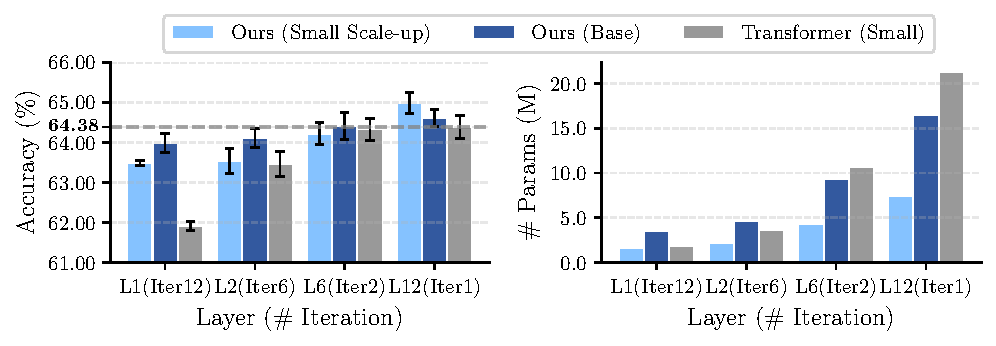
\includegraphics[width=0.9\linewidth]{figures/bar_plot_with_upper_bound.pdf}
    % \vskip -.1in
    \caption{Top-1 accuracy (\emph{Left}) and model parameters (\emph{Right}) on CIFAR-100 with different layer-iteration trade-offs. Our model (Base) consistently surpasses Transformer, even its upper bound performance, with parameter efficiency. Error bars represent standard deviation over five runs.}
    \label{fig:bar plot cifar10}
\end{figure}
% \todo{need to adapt trade-off figure to the newest setting}

\subsection{Image Classification}
\label{section:image classification}



% \begin{table*}[htbp]
%     \centering
%     \begin{minipage}{0.7\textwidth}
%     \centering
%     \caption{Top-1 accuracy on image classification. Models are under the same hidden dimension and 1 layer with 12 iterations. Scaling up our model to match Transformer's parameters gives better performance. Parameters are measured on CIFAR-10.}
%     \label{tab:classification}
%         % \resizebox{\linewidth}{!}{
%         % \begin{tabular}{ll}
%         \begin{tabularx}{\linewidth}{lllll}
%         \toprule
%         \multirow{2}{*}{Models}  & \multirow{2}{*}{Config ($\#$ Params)} & \multicolumn{3}{c}{Dataset}\\
%         \cmidrule(lr){3-5}
%          &  & CIFAR-10 & CIFAR-100 & IM-100\\
%         \midrule
%         Transformer  & Small (1.8 M) & 89.91 & 62.09 &  \textbf{xx}\\
%         \textsc{CRATE}-T \citep{hu2024an}  & Small (xx M) & xx &  xx & xx \\
%         \textsc{CRATE} \citep{yu2023white} & Small (0.47 M) & 87.91 & 60.57 & xx\\
%         Energy Transformer \citep{hoover2024energy} & Small (0.91 M) & 75.78 & 52.86 & xx\\
%         Ours  & Small (0.97 M) & 88.66 & 61.28 & 54.78\\
%         \midrule
%         % \textsc{CRATE} & Base (2.37466 M) & 84.94 & 53.75 & xxx  \\
%         Ours  & Small Scale-up (1.5 M) & \textbf{90.11} & \textbf{63.24} & 55.98\\
%         \bottomrule
%         \end{tabularx}
%         % \end{tabular}
%         % }
%     \end{minipage}%
%     \hspace{\fill}
%     \begin{minipage}{0.28\textwidth}
%     \centering
%     \caption{Model configuration for solving Sudoku.}
%     \label{tab:alternative design} 
%         % \resizebox{\linewidth}{!}{
%         % \begin{tabular}{ll}
%         \begin{tabularx}{\linewidth}{ll}
%             \toprule
%             Ours  & Value \\
%             \midrule
%             Ours & 10 \\
%             \midrule
%             Ours & 5.20 M \\
%             \bottomrule
%         \end{tabularx}
%         % \end{tabular}
%         % }
%     \end{minipage}
% \end{table*}

\paragraph{Setups \& Results.}
We also compare \textsc{Hyper-SET} on CIFAR-10/100, ImageNet-100,\footnote{We use a subset of ImageNet-1K from \href{https://github.com/HobbitLong/CMC/blob/master/imagenet100.txt}{\text{https://github.com/HobbitLong/CMC/blob/master/imagenet100.txt}}} and the full ImageNet-1K against ViTs, \textsc{CRATE} \citep{yu2023white} its variant \textsc{CRATE}-T that aims for more faithful implementations \citep{hu2024an}, and Energy Transformer \citep{hoover2024energy}. Detailed setups are in Appendix~\ref{section:image classification setup}. 

% \begin{table}[htbp]
% \caption{Top-1 accuracy ($\%$) for image classification with single-layer recurrent-depth models. Parameters are measured on ImageNet-1K. All models are trained from scratch on the listed datasets. }
% \label{tab:classification}
% \centering
% \resizebox{\linewidth}{!}{
% \begin{tabular}{lcccccc}
% \toprule
% \multirow{2}{*}{Models}  & \multirow{2}{*}{Width $d$} & \multirow{2}{*}{$\#$ Params} &\multicolumn{4}{c}{Dataset}\\
% \cmidrule(lr){4-7}
%  &  & & CIFAR-10 & CIFAR-100 & IN-100 & IN-1K\\
% \midrule
% Transformer  & 384 & 2.38 M & 89.90 & 61.89 &  69.44 & \textbf{66.94}\\
% \textsc{CRATE}-T \citep{hu2024an}  & 896 & 3.04 M & 87.54&  60.23& 68.16 & 57.89\\
% \textsc{CRATE} \citep{yu2023white} & 768 & 3.00 M & 84.81& 58.22& 68.52 & 57.00\\
% Energy Transformer \citep{hoover2024energy} & 512 & 2.39 M & 76.39& 50.60 & 36.68 & 34.24\\
% \midrule
% Ours  & 512 & 2.39 M & \textbf{90.11}& 63.41 & \textbf{70.16} & 62.76\\
% % \textsc{CRATE} & Base (2.37466 M) & 84.94 & 53.75 & xxx  \\
% Ours  & 640 & 3.40 M & 89.96 & \textbf{64.60} & 69.31 & 66.21\\
% \bottomrule
% \end{tabular}
% }
% \end{table}

% \begin{table}[htbp]
% \caption{Top-1 accuracy ($\%$) for image classification with single-layer recurrent-depth models. Parameters are measured on ImageNet-1K. All models are trained from scratch on the listed datasets.}
% \label{tab:classification}
% \centering
% \sisetup{detect-weight=true, detect-family=true} % Setup for bolding in S columns
% \resizebox{0.95\linewidth}{!}{
% \begin{tabular}{l c S[table-format=1.2] S[table-format=2.2] S[table-format=2.2] S[table-format=2.2] S[table-format=2.2]}
% \toprule
% \multirow{2.5}{*}{\thead{Model}} & \multirow{2.5}{*}{\shortstack{\thead{Width}\\($d$)}} & \multirow{2.5}{*}{\shortstack{\thead{Width}\\($d$)}} & \multicolumn{4}{c}{\thead{Dataset}} \\
% \cmidrule(lr){4-7}
%  & &  & {CIFAR-10} & {CIFAR-100} & {IN-100} & {IN-1K} \\
% \midrule
% \multicolumn{7}{l}{\emph{Baselines}} \\
% Transformer & 384 & 2.38 & 89.90 & 61.89 & 69.44 & \bfseries 66.94 \\
% \textsc{CRATE}-T \citep{hu2024an} & 896 & 3.04 & 87.54 & 60.23 & 68.16 & 57.89 \\
% \textsc{CRATE} \citep{yu2023white} & 768 & 3.00 & 84.81 & 58.22 & 68.52 & 57.00 \\
% Energy Trans. \citep{hoover2024energy} & 512 & 2.39 & 76.39 & 50.60 & 36.68 & 34.24 \\
% \midrule
% \multicolumn{7}{l}{\emph{Our Method}} \\
% \textbf{\textsc{Hyper-SET}} ($d=512$)& 512 & 2.39 & \bfseries 90.11 & 63.41 & \bfseries 70.16 & 62.76 \\
% \textbf{\textsc{Hyper-SET}} ($d=640$)& 640 & 3.40 & 89.96 & \bfseries 64.60 & 69.31 & 66.21 \\
% \bottomrule
% \end{tabular}
% }
% \end{table}

\begin{table}[htbp]
\caption{Top-1 accuracy ($\%$) for image classification with single-layer recurrent-depth models. Parameters are measured on ImageNet-1K. All models are trained from scratch on the listed datasets.}
\label{tab:classification}
\centering
\resizebox{\linewidth}{!}{
\begin{tabular}{lcccccc}
\toprule
\multirow{2.5}{*}{\textbf{Model}} & \multirow{2.5}{*}{\shortstack{\textbf{Width}\\\textbf{$d$}}} & \multirow{2.5}{*}{\shortstack{\textbf{\# Params}\\(M)}} & \multicolumn{4}{c}{\textbf{Dataset}} \\
\cmidrule(lr){4-7}
 & & & CIFAR-10 & CIFAR-100 & IN-100 & IN-1K \\
\midrule
Transformer & 384 & 2.38 & 89.90 & 61.89 & 69.44 & \textbf{66.94} \\
\textsc{CRATE}-T \citep{hu2024an} & 896 & 3.04 & 87.54 & 60.23 & 68.16 & 57.89 \\
\textsc{CRATE} \citep{yu2023white} & 768 & 3.00 & 84.81 & 58.22 & 68.52 & 57.00 \\
Energy Transformer \citep{hoover2024energy}& 512 & 2.39 & 76.39 & 50.60 & 36.68 & 34.24 \\
\midrule
\textsc{Hyper-SET} (Ours) & 512 & 2.39 & \textbf{90.11} & 63.41 & \textbf{70.16} & 62.76 \\
\textsc{Hyper-SET} (Ours) & 640 & 3.40 & 89.96 & \textbf{64.60} & 69.31 & 66.21 \\
\bottomrule
\end{tabular}
}
\end{table}

Table~\ref{tab:classification} shows that, under properly parameter-aligned settings, our model surpasses others on CIFAR-10/100 and ImageNet-100 but lags behind Transformer on large-scale ImageNet-1K. Notably, our architecture achieves a higher width-parameter ratio compared to Transformer, meaning more parameter-efficient under the same width.\footnote{We compare the parameter efficiency and computational cost in Appendix~\ref{section:param and time}.} When scaling up the width $d$, our model can narrow the performance gap to Transformer. This implies that our principled model suits better under a resource-constrained setting as its inherent structural biases could limit its scaling on large datasets.

%achieves the best results.  
\paragraph{Layer-Iteration Trade-off.}
So far, the classification is conducted using a one-layer model. A natural question is how well the model performs when stacking multiple layers with different parameters. To see this, we first train a Transformer with 12 layers—equivalent in effective depth to one layer with 12 iterations—as an upper bound. We then vary the number of distinct layers and their iterations while keeping total depth constant, effectively introducing flexibility to the basis vectors. 

% Then, we vary the ratio of distinct layers and their respective iterations while maintaining the effective depth. This configuration can be interpreted as adding flexibility to the basis vectors. 
%which the energy is conditioned on. 

In Figure~\ref{fig:bar plot cifar10}, our scaled-up $\texttt{small}$ model has parameter efficiency across varied layer-iteration ratios, with this strength intensifying as more independent layers are trained. However, its architectural efficiency limits scalability beyond two layers. Scaling to the $\texttt{Base}$ configurations enables our model to consistently outperform Transformer, exceeding the upper bound while retaining less parameters.
 % In Figure~\ref{fig:bar plot cifar10}, our scaling-up $\texttt{small}$ model has parameter-efficiency at varied layer-iteration ratios, and this strength is greatly sharpened when more independent layers are learned. However, this architectural efficiency limits its scalability beyond two layers. Yet, by scaling to the $\texttt{Base}$ configuration, ours consistently outperforms Transformer even surpassing the upper bound while retaining parameter efficiency.
 %The $\texttt{Base}$ model is still parameter-efficient with more layers. 
 
% \paragraph{Energy, Effective Rank \& Average Angle}
% The hyperspherical energy monotonically decreases as in Figure~\ref{fig:energy} (Bottom) for our $\texttt{Small}$ model with effective rank and average angle mirroring trends from the Sudoku experiment in Figure~\ref{fig:angle}. Complete results are in Appendix~\ref{section:rank angle cifar10 complete}.


% \begin{table}[htbp]
% \caption{Top-1 Accuracy on Image Classification.}
% \label{tab:classification}
% \centering
% \resizebox{\linewidth}{!}{
% \begin{tabular}{llcc}
% \toprule
% \multirow{2}{*}{Datasets}  & \multirow{2}{*}{Models} & \multicolumn{2}{c}{Configuration}\\
% \cmidrule(lr){3-4}
%  &  & Tiny & Base\\
% \midrule
% \multirow{3}{*}{CIFAR-10}  & Transformer &  xx &  xx\\
%                               & \textsc{CRATE} &  xx & xx  \\
%                              & Ours  & xx & xx \\
% \multirow{3}{*}{CIFAR-100}  & Transformer &  xx &  xx\\
%                               & \textsc{CRATE} &  xx & xx  \\
%                              & Ours  & xx & xx \\
% \multirow{3}{*}{Imagenet-100}  & Transformer &  xx &  xx\\
%                               & \textsc{CRATE} &  xx & xx  \\
%                              & Ours  & xx & xx \\
% \bottomrule
% \end{tabular}
% }
% \end{table}
% \vspace{-0.7cm}

\paragraph{Non-Recurrent Scenarios.} 
To demonstrate the practicality in the non-recurrent settings, which are more common in large-scale applications, we further provide comparisons in a 12-layer non-recurrent setting in Table~\ref{tab:classification multi-layer}, where we report results on CIFAR-10/100 with fine-tuning or training from scratch and on large-scale ImageNet-1K. The ImageNet-1K pretraining setup follows Table~\ref{tab:classification}, with fine-tuning batch size 256, epochs 50, learning rate 1e-4, and weight decay 1e-5. Our model performs comparably as standard Transformers while being more parameter-efficient, and this parameter reduction constantly grows when stacking more distinct layers, as shown in Figure~\ref{fig:bar plot cifar10}, thanks to our parsimonious design. This suggests that \textsc{Hyper-SET} potentially preserves the benefit of scaling in Transformers when extended practically, while being more useful in resource-constrained settings where model size matters, further underscoring its promise in practical scenarios.

% Our model can actually scale almost equally well as standard Transformer while being more parameter-efficient. This suggests our model can have the benefit of scaling in Transformer when extended practically, meanwhile being more useful in resource-constrained settings.


% This suggests our model can have the benefit of scaling in Transformer when extended practically, meanwhile being more useful in resource-constrained settings.

% \begin{table}[htbp]
% \caption{Top-1 accuracy ($\%$) for image classification with 12-layer non-recurrent-depth models. Parameters are measured on ImageNet-1K. $^\dagger$ means first pretraining on ImageNet-1K and then fine-tuning on CIFAR-10/100.}
% \label{tab:classification multi-layer}
% % \vskip -.1in
% \centering
% \resizebox{\linewidth}{!}{
% % \arrayrulecolor{blue}
% \begin{tabular}{lccccccc}
% \toprule
% \multirow{2}{*}{Models}  & \multirow{2}{*}{Width $d$} & \multirow{2}{*}{$\#$ Params} &\multicolumn{5}{c}{Dataset}\\
% \cmidrule(lr){4-8}
%  &  & & CIFAR-10 & CIFAR-100 & CIFAR-10$^\dagger$ & CIFAR-100$^\dagger$ & IN-1K\\
% \midrule
% Transformer  & 384 & 21.86 M & 87.44 & 62.84 & \textbf{96.95} & \textbf{83.10} & \textbf{67.90}\\
% \textsc{CRATE} \citep{yu2023white} & 512 & 10.28 M & 88.76  & 63.94 & 94.18 & 77.39 & 60.69\\
% \midrule
% Ours  & 512 & 8.17 M & \textbf{88.82} & \textbf{64.98} & 95.76 & 80.89 & 66.26\\
% Ours  & 768 & 17.56 M & 88.53 & 64.16  & 96.47 & 82.60 & 67.20\\
% % \textsc{CRATE} & Base (2.37466 M) & 84.94 & 53.75 & xxx  \\
% % Ours  & 640 & 3.40 M & 89.96 & \textbf{64.60} & 66.21\\
% \bottomrule
% \end{tabular}
% % \arrayrulecolor{black}
% }
% \end{table}


\begin{table}[htbp]
\caption{Top-1 accuracy ($\%$) for image classification with 12-layer non-recurrent-depth models. Parameters are measured on ImageNet-1K. $^\dagger$ means first pretraining on ImageNet-1K and then fine-tuning on CIFAR-10/100.}
\label{tab:classification multi-layer}
\centering
\resizebox{\linewidth}{!}{
\begin{tabular}{lccccccc}
\toprule
\multirow{2.5}{*}{\textbf{Model}} & \multirow{2.5}{*}{\shortstack{\textbf{Width}\\\textbf{$d$}}} & \multirow{2.5}{*}{\shortstack{\textbf{\# Params}\\(M)}} & \multicolumn{5}{c}{\textbf{Dataset}} \\
\cmidrule(lr){4-8}
 & & & CIFAR-10 & CIFAR-100 & CIFAR-10$^\dagger$ & CIFAR-100$^\dagger$ & IN-1K \\
\midrule
Transformer  & 384 & 21.86  & 87.44 & 62.84 & \textbf{96.95} & \textbf{83.10} & \textbf{67.90}\\
\textsc{CRATE} \citep{yu2023white} & 512 & 10.28  & 88.76  & 63.94 & 94.18 & 77.39 & 60.69\\
\midrule
\textsc{Hyper-SET} (Ours)  & 512 & 8.17  & \textbf{88.82} & \textbf{64.98} & 95.76 & 80.89 & 66.26\\
\textsc{Hyper-SET} (Ours) & 768 & 17.56  & 88.53 & 64.16  & 96.47 & 82.60 & 67.20\\
\bottomrule
\end{tabular}
}
\end{table}


\subsection{Masked Image Modeling}
\paragraph{Setups \& Results.}
Masked image modeling has recently regained its traction for autoregressive generation \citep{li2023mage,li2024autoregressive}, framed as recovering images from $100\%$ masking. Due to its high computational demand, we attempt to demonstrate the power of our one-layer model specifically for image reconstruction on ImageNet-100. We build on prior work \citep{chang2022maskgit} and use the open-source repository.\footnote{\href{https://github.com/valeoai/Maskgit-pytorch}{\text{https://github.com/valeoai/Maskgit-pytorch}}} Concrete settings are in Appendix~\ref{section:masked image modeling setup}, with additional results and visualization in Appendix~\ref{section:additional results of masked image modeling}.

% \begin{wrapfigure}{r}{0.5\textwidth}
% \centering
% \includegraphics[width=\linewidth]{visualization.pdf}
% \caption{Visual Comparison on Masked Image Modeling on ImageNet 256$\times$256. Our model, when scaling to Transformer scale with additional compute, can achieve similar reconstruction quality when masking ratio $=40\%$.}
% \label{fig:visualization}
% \end{wrapfigure}

Table~\ref{tab:masked image modeling} unveils that, under the same number of iterations, our model significantly reduces parameters but lags behind Transformer on all metrics. If we further increase its iterations and the width of feedforward module $M$ to 8$d$, it can fill in the performance gap but at the cost of more computation.

\begin{table}[htbp]
\caption{Comparisons of masked image modeling performance on ImageNet-100 (5k). While our model is more compact, scaling the feedforward module width ($M$) allows it to match Transformer performance. All models use a single layer.}
\label{tab:masked image modeling}
\centering
\resizebox{\textwidth}{!}{
\begin{tabular}{l c c S[table-format=1.2] S[table-format=2.3] S[table-format=1.3] S[table-format=1.3] S[table-format=1.3] S[table-format=2.3]}
\toprule
\textbf{Model} & \textbf{Iters} & \textbf{FF Ratio $M$} & {\textbf{\# Params (M)}} & \textbf{PSNR ($\uparrow$)} & \textbf{SSIM ($\uparrow$)} & \textbf{MS-SSIM ($\uparrow$)} & \textbf{LPIPS ($\downarrow$)} & \textbf{FID ($\downarrow$)} \\
\midrule
Transformer & 12 & $4d$ & 8.85 & 15.953 & \textbf{0.417} & \textbf{0.599} & \textbf{0.327} & \textbf{43.428} \\
\textsc{Hyper-SET} (Ours) & 12 & $1d$ & 3.94 & 15.713 & 0.411 & 0.576 & 0.358 & 59.841 \\
\textsc{Hyper-SET} (Ours) & 24 & $8d$ & 8.07 & \textbf{15.955} & \textbf{0.417} & 0.596 & 0.332 & 45.174 \\
\bottomrule
\end{tabular}
}
\end{table}

% \begin{figure}[!tbp]
%     \centering
%     \includegraphics[width=\linewidth]{visualization.pdf}
%         % \vskip -.1in
%     \caption{Visual Comparison on Masked Image Modeling on ImageNet 256$\times$256. Our model, when scaling to Transformer scale with additional compute, can achieve similar reconstruction quality when masking ratio $=40\%$.}
%     \label{fig:visualization}
% \end{figure}


% \begin{figure}[tbp]
%   \centering
%   \begin{subfigure}[t]{0.49\textwidth}
%     \centering
%     
\includegraphics[width=\linewidth]{energy_sudoku.pdf}
%     \caption{Sudoku}
%     \label{fig:energy sudoku}
%   \end{subfigure}
%   \hfill % Adds horizontal space between subfigures
%   \begin{subfigure}[t]{0.49\textwidth}
%     \centering
%     \includegraphics[width=\linewidth]{energy.pdf}
%     \caption{CIFAR-10}
%     \label{fig:energy cifar10}
%   \end{subfigure}
%   \caption{The energy of both the attention and feedforward module decreases on Sudoku (\emph{Left}) and CIFAR-10 (\emph{Right}), without hard constraints on the sign of the step size. This suggests the layer aligns well with the optimization objective. Normalization is first applied to meet the condition in \Eqref{eq:5} before computing the energy.}
%   \label{fig:energy}
% \end{figure}


% \begin{wrapfigure}{r}{0.5\textwidth}
% \centering
% 
\includegraphics[width=\linewidth]{energy_sudoku.pdf}
% \includegraphics[width=\linewidth]{energy.pdf}
% \caption{The energy of both the attention and feedforward module decreases on Sudoku (\emph{Top}) and CIFAR-10 (\emph{Bottom}), without hard constraints on the sign of the step size. This suggests the layer aligns well with the optimization objective. Normalization is first applied to meet the condition in \Eqref{eq:5} before computing the energy.}
% \label{fig:energy}
% \end{wrapfigure}
\begin{figure}[tbp]
  \centering
    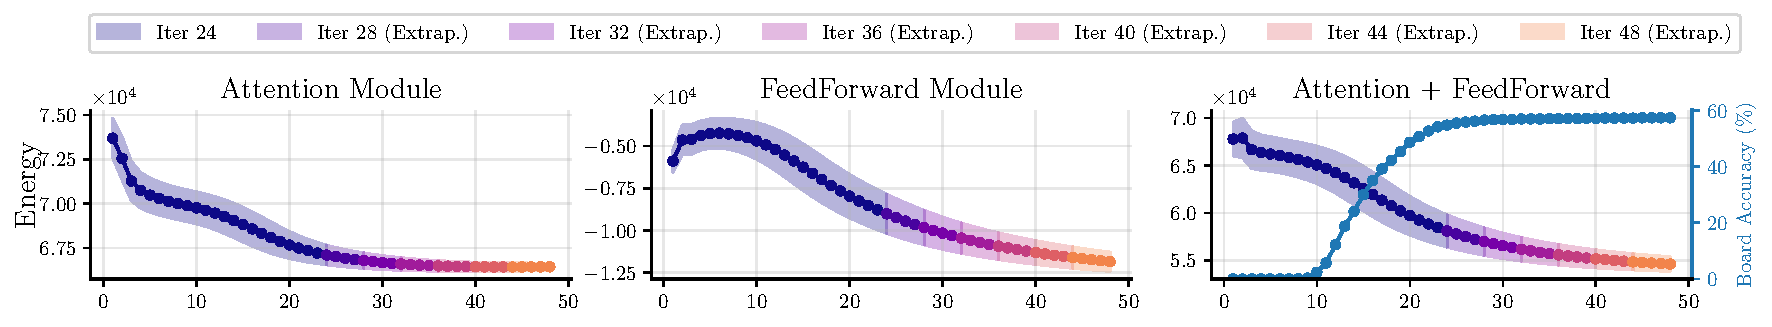
\includegraphics[width=\linewidth]{figures/energy_sudoku_with_acc.pdf}
    % \caption{Sudoku}
    % \label{fig:energy sudoku}
    % \vspace{-10pt}
    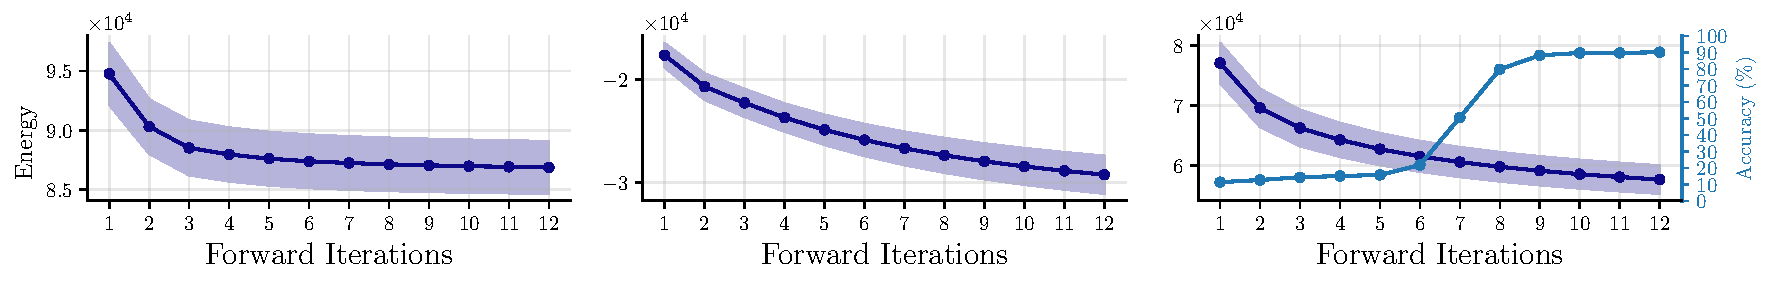
\includegraphics[width=\linewidth]{figures/energy_with_acc.pdf}
    % \caption{CIFAR-10}
    % \label{fig:energy cifar10}
    % \vskip -.1in
  \caption{The attention and feedforward energy decrease on Sudoku (\emph{Top}) and CIFAR-10 (\emph{Down}) even without sign constraints on step sizes. This suggests the layer aligns well with the optimization objective. Normalization is first applied to meet constraints in \Eqref{eq:5} before computing the energy. In the right subfigure, the decrease in the overall energy corresponds to the increase in performance.}
  \label{fig:energy}
\end{figure}
\subsection{Energy Evolution, Effective Rank and Average Angle}


Figure~\ref{fig:energy} shows energy trajectories of the attention ($E_{\text{ATTN}}$) and feedforward module ($E_{\text{FF}}$). Even without a positive threshold for step sizes $\alpha_t$ and $\gamma_t$, the energy on Sudoku still decreases within training iterations and extrapolates smoothly beyond them, indicating strong generalization of learned step sizes. On CIFAR-10, our designed energy exhibits a monotonic decline as well.

%for the $\texttt{Small}$ model too.

To verify our subspace uniformity objective, we track two metrics—\emph{effective rank} and \emph{average angle}—defined in Appendix~\ref{section:definition}. As shown in Figure~\ref{fig:rank angle}, the subspace effective rank steadily increases while the full rank remains unchanged. Meanwhile, average angles between tokens approach orthogonality, aligning with our goal to prevent entropy collapse. Full results and comparisons with parameter-sharing Transformer are in Appendix~\ref{section:rank angle sudoku cifar10 complete}.

\begin{figure}[tbp]
  \centering
  \begin{subfigure}[t]{0.49\textwidth}
    \centering
    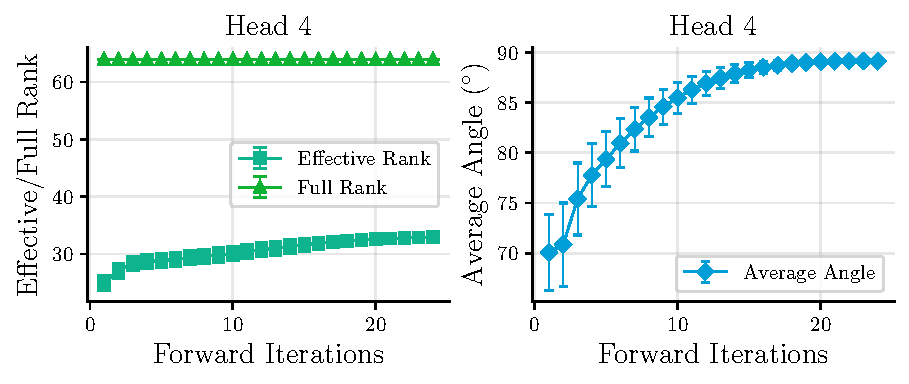
\includegraphics[width=\linewidth]{figures/rank_angle_sudoku.pdf}
    % \vspace{-20pt}
    % \vskip -0.05in
    \caption{Sudoku.}
    \label{fig:rank}
  \end{subfigure}
  \hfill % Adds horizontal space between subfigures
  \begin{subfigure}[t]{0.49\textwidth}
    \centering
    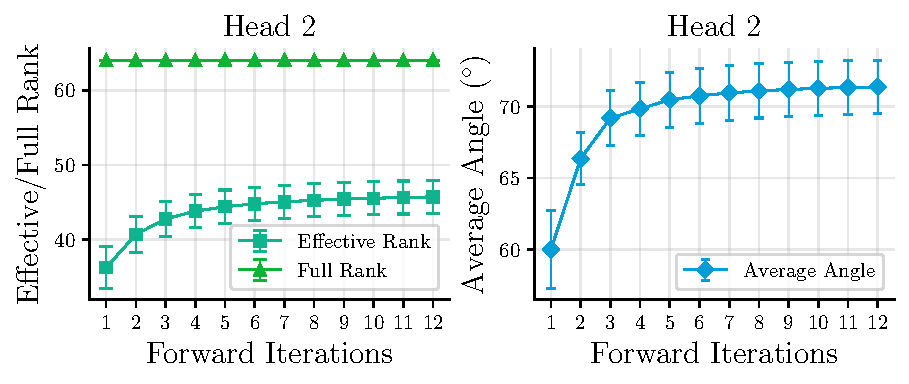
\includegraphics[width=\linewidth]{figures/rank_angle-v2.pdf}
    % \vskip -.1in
    \caption{CIFAR-10.}
    \label{fig:angle}
  \end{subfigure}
   % \vskip -.1in
  \caption{The effective rank and average angle of tokens projected to one subspace gradually increase, suggesting a larger volume spanned by these tokens. Results are from Sudoku test dataset \citep{palm2018recurrent} (\emph{Left}) and CIFAR-10 validation set (\emph{Right}).}
  \label{fig:rank angle}
\end{figure}
% Likewise, the average angle between latent tokens grows from $\sim70^\circ$ toward near orthogonality. This implies that latent tokens occupy maximal hyperspherical volume and prevent entropy collapse, aligning with our objective. Full results are in Appendix~\ref{section:rank angle sudoku cifar10 complete}.

% To further validate our motivation for subspace uniformity, we quantify tokens separation via two metrics: \emph{effective rank} and \emph{average angle} (see Appendix~\ref{section:definition} for definitions). Figure~\ref{fig:rank angle} reveals that the effective rank steadily increases within the subspace while the full rank remains unchanged. This trend is paralleled by the average angle, which grows from around $70^{\circ}$ to near orthogonality. This implies that tokens in the low-dimensional space occupy maximal hyperspherical volume and prevent entropy collapse, corroborating our design goal. Full results are in Appendix~\ref{section:rank angle sudoku cifar10 complete}.

% To further validate our motivation to enhance distributional uniformity within subspaces, we employ two metrics to quantify the separation of tokens: \emph{effective rank} and \emph{average angle} (see Appendix~\ref{section:definition} for definitions). Figure~\ref{fig:rank angle} reveals that as the forward optimization proceeds, the effective rank steadily increases within the subspace while the full rank remains unchanged. This trend is paralleled by the average angle, which grows from around $70^{\circ}$ to near orthogonality. This implies that tokens in the low-dimensional space occupy maximal hyperspherical volume and preserve entropy collapse, corroborating our design goal. Full results are in Appendix~\ref{section:rank angle sudoku cifar10 complete}.

%It corroborates our initial design goal of the attention energy $E_{\text{ATTN}}$.
% \todo{comparison with other architectures}

% \begin{wraptable}{l}{0.49\textwidth}
% \centering
% \caption{Alternative designs on key components measured by top-1 accuracy.}
% \label{tab:alternative design}
% \resizebox{\linewidth}{!}{
% \begin{tabular}{llll}
% \toprule
% \multirow{2}{*}{Components}  & \multirow{2}{*}{Alternative Designs} & \multicolumn{2}{c}{Dataset}\\
% \cmidrule(lr){3-4}
%  &  & CIFAR-10 & CIFAR-100 \\
% \midrule
% \multirow{3}{*}{$E_{\text{ATTN}}$} & Bi-Softmax Attention (Ours)& \textbf{90.11} & \textbf{63.41} \\
%                                    & Sigmoid Attention & 85.93 & 59.72 \\
%                                    & Linear Attention & 84.88 & 56.97 \\
% \midrule
% \multirow{3}{*}{$E_{\text{FF}}$} & ReLU FF (Ours) & \textbf{90.11} &\textbf{63.41} \\
%                                    & Softmax FF & 88.20 & 62.44 \\
%                                    & Gated FF (sigmoid) & 84.99 & 59.29 \\
% \midrule
% \multirow{3}{*}{Step Size} & Learning Step Size (Ours)& \textbf{90.11} & \textbf{63.41} \\
%                            & $\alpha_t=\gamma_t$ = 0.5 & 25.81 & 57.92 \\
%                            % & $\alpha_t=\gamma_t$ = 0.2 & xx & xx \\
%                            & $\alpha_t=\gamma_t$ = 0.1 & 81.45 & 58.29 \\
% \bottomrule
% \end{tabular}
% }
% \end{wraptable}


% \begin{wraptable}{r}{0.49\textwidth}
% \centering
% \caption{Imagenet-100 accuracy of \textsc{Hyper-SET} under different matrix rank within LoRA. Layer-wise LoRA introduces flexibility in the computation at each iteration.}
% \label{tab:layer-wise lora}
% % \resizebox{\linewidth}{!}{
% \begin{tabular}{lll}
% \toprule
% Rank  & $\#$ Params & Accuracy (\%)\\
% \midrule
% 4 & xx M & xx\\
% 8 & xx M & xx\\
% 16 & xx M & xx\\
% \bottomrule
% \end{tabular}
% % }
% \end{wraptable}

\begin{table*}[htbp]
    \centering
    \begin{minipage}[t]{0.52\textwidth} % 0.55
    \centering
    \caption{Alternative design instantiations on key components measured by top-1 accuracy ($\%$).}
    \vspace{-5pt}
    \label{tab:alternative design}
        \resizebox{\linewidth}{!}{
        \begin{tabular}{llcc}
        % \begin{tabularx}{\linewidth}{llll}
           \toprule
            \textbf{Components}  & \textbf{Alternative Designs} & \textbf{CIFAR-10} & \textbf{CIFAR-100} \\
            \midrule
            \multirow{3}{*}
            {$E_\text{ATTN}$} & Bi-Softmax Attention (Default)& \textbf{90.11} & \textbf{63.41} \\
               & Sigmoid Attention & 85.93 & 59.72 \\
               & Linear Attention & 84.88 & 56.97 \\
            \midrule
            \multirow{3}{*}{$E_{\text{FF}}$} & ReLU FF (Default) & \textbf{90.11} &\textbf{63.41} \\
               & Softmax FF & 88.20 & 62.44 \\
               & Gated FF  & 84.99 & 59.29 \\
            \midrule
            \multirow{3}{*}{Step Size} & Learned Step Size (Default)& \textbf{90.11} & \textbf{63.41} \\
               & $\alpha_t=\gamma_t$ = 0.5 & 25.81 & 57.92 \\
               % & $\alpha_t=\gamma_t$ = 0.2 & xx & xx \\
               & $\alpha_t=\gamma_t$ = 0.1 & 81.45 & 58.29 \\
            \bottomrule
        % \end{tabularx}
        \end{tabular}
        }
    \end{minipage}%
    \hfill
    \begin{minipage}[t]{0.46\textwidth} % 0.44
    \centering
    \caption{ImageNet-100 accuracy ($\%$) of \textsc{Hyper-SET} under different matrix rank ($r$) in LoRA. Depth-wise LoRA introduces representation flexibility at each iteration.}
    \vspace{2pt}
    \label{tab:layer-wise lora}
        \resizebox{\linewidth}{!}{
        \begin{tabular}{lcc}
        % \begin{tabularx}{\linewidth}{lll}
            \toprule
            \textbf{Model}  & \textbf{$\#$ Params (M)} & \textbf{Accuracy}\\
            \midrule
            \textsc{Hyper-SET} (Ours) & 1.93  & 70.16 \\
            + depth-wise LoRA ($r=4$) & 2.03 & 70.36\\
            + depth-wise LoRA ($r=8$) & 2.13 & 70.40\\
            + depth-wise LoRA ($r=16$) & 2.33 & 70.56\\
            + depth-wise LoRA ($r=32$) & 2.72 & \textbf{72.20}\\
            \bottomrule
        % \end{tabularx}
        \end{tabular}
        }
    \end{minipage}
\end{table*}

\subsection{Alternative Designs and Scalability}
% A key strength of our formulation~\Eqref{eq:mle ultimate form} is its generality: it is not limited to a single instantiation, but enables a spectrum of variants through alternative energy functions. By generalizing the attention energy with kernel functions, we can induce novel attention structures and even linear attention. Similarly, a gating mechanism can also arise from generalizing feedforward energy. Table~\ref{tab:alternative design} shows their evaluation along with different fixed step sizes. More elaboration is provided in Appendix~\ref{section:alternative designs}. 

% To further enhance the scalability of \textsc{Hyper-SET} while preserving its compact parameterization, we introduce an extension that adds lightweight flexibility to the shared layer parameters, inspired by~\citep{bae2025relaxed}. We insert learnable low-rank adapters for each forward iteration to modulate the shared weights in a depth-specific manner during training. Figrue~\ref{tab:layer-wise lora} shows that this flexibility adds up to the performance. We provide setup and other scaling results in Appendix~\ref{section:scalability}. 
A key strength of our formulation~\Eqref{eq:mle ultimate form} lies in its generality—it supports a broad spectrum of model variants through alternative energy functions. For example, replacing the attention energy with a kernel-based function yields novel attention mechanisms, including linear attention. Similarly, gating in feedforward layers naturally arises by generalizing the feedforward energy. Table~\ref{tab:alternative design} shows the performance of these variants and results with different fixed step sizes, with details in Appendix~\ref{section:alternative designs}

To improve scalability with compact parameterizations, we introduce a lightweight extension inspired by~\citet{bae2025relaxed}, where learnable low-rank adapters are added at each forward iteration to modulate shared weights. This depth-wise adaptation, shown in Table~\ref{tab:layer-wise lora}, enhances performance without significantly increasing parameter count. Setups and additional scaling results on image and text modalities are included in Appendix~\ref{section:scalability}.